\documentclass[journal]{IEEEtran}

\usepackage{cite}
\usepackage{graphicx}
\usepackage{amsmath}
\usepackage{url}
\usepackage{booktabs}
\usepackage{xcolor}

\begin{document}

\title{Building VHDL Processors with Claude Code:\\From 16-Bit to 64-Bit FPU}

\author{George~Teifel,~\IEEEmembership{}
        and~Siamak~Tavakoli%
\thanks{G.~Teifel (corresponding author, e-mail: gteifel@unm.edu; ORCID: https://orcid.org/0009-0006-4371-6799) and S.~Tavakoli (e-mail: stavakoli@unm.edu) are with the Department of Electrical and Computer Engineering, University of New Mexico, Albuquerque, NM 87131, USA.}%
% TODO: add Tavakoli ORCID if he has one
}

\maketitle

\begin{abstract}
Manual register-transfer level (RTL) design is labor-intensive and demands expertise in both digital logic and synthesis tool chains. This paper presents a skill-based methodology for AI-assisted hardware description language (HDL) generation with Claude Code. A custom skill was built by merging two community-contributed FPGA design skills and adding three capabilities: a simulation-first test-driven development (TDD) mandate, live documentation retrieval through Context7 MCP integration, and Vivado version-aware code generation. Using this skill, six RISC-V processor designs were generated in a single session---three in Verilog and three in VHDL---spanning 16-bit educational cores (RV32I subset), 64-bit integer processors (RV64I), and a 64-bit processor with an IEEE 754 double-precision floating-point unit (RV64IFD). The most complex variant implements 68 instructions and 28 FPU operations in a 5-stage pipeline, consuming 12,969 look-up tables (LUTs) and 18 DSP48E1 slices on a Xilinx Artix-7 XC7A35T. The TDD workflow caught 10 floating-point bugs in the initial generation and produced a 48\% LUT reduction, from roughly 25,000 to 12,969 LUTs. Formal verification with SystemVerilog Assertions and SymbiYosys bounded model checking was then added, proving correctness properties for ALU operations, FPU IEEE 754 special-value handling, pipeline hazard detection, and memory bus protocols in all three variants. All designs were validated on a Digilent Basys 3 board. Domain-specific skill engineering materially improves the quality and completeness of AI-generated HDL.
\end{abstract}

\begin{IEEEkeywords}
RISC-V, FPGA, hardware description language, large language model, test-driven development, formal verification, IEEE 754, Claude Code
\end{IEEEkeywords}

\section{Introduction}

Register-transfer level (RTL) processor design requires expertise in computer architecture, hardware description languages, synthesis tool chains, and verification methodology. Even experienced engineers need weeks to months to produce a verified processor targeting a specific field-programmable gate array (FPGA) platform~\cite{patterson2017cod}. Large language models (LLMs) now generate software code competently, but their application to HDL has stayed exploratory and prior results have been confined to small designs~\cite{thakur2023date, blocklove2023chipchat, pearce2020dave, sun2024hdlgen, zhao2025resbench}.

The gap between LLM-generated HDL and practical processor design is wide. Thakur et al.~\cite{thakur2023date} benchmarked LLMs on small Verilog module tasks at DATE 2023: the best model hit 25.9\% syntactic correctness and only 6.5\% functional correctness, on isolated modules such as counters, adders, and FIFOs rather than complete processors. Pearce et al.~\cite{pearce2020dave} set early baselines at MLCAD 2020 with DAVE, generating small Verilog modules from English descriptions but never attempting system-level designs. Blocklove et al.~\cite{blocklove2023chipchat} reached the most ambitious prior result at MLCAD 2023 with Chip-Chat, an 8-bit accumulator-based microprocessor billed as the first wholly AI-written HDL for tapeout. It had an 8-bit datapath, no pipeline, no FPU, and a minimal instruction set. Sun et al.~\cite{sun2024hdlgen} later used ChatGPT-3.5 to generate an RV32I processor in VHDL and Verilog, but the design was limited to 32-bit integer operations with no FPU and no dual-language parity. Zhao et al.~\cite{zhao2025resbench} introduced ResBench with 56 FPGA benchmarks measuring resource efficiency of LLM-generated designs, again at the module level.

Several efforts have pushed artificial intelligence (AI)-assisted hardware design further since those works. Liu et al.~\cite{liu2024rtlcoder} proposed RTLCoder, an open-source framework that fine-tunes a lightweight LLM for Verilog generation and outperforms GPT-3.5 on RTL benchmarks with far fewer parameters. The generated designs remain module-level (counters, ALUs, FIFOs). NVIDIA's ChipNeMo~\cite{chipnemo2024} adapted a foundation LLM for chip design tasks including code generation, an engineering assistant chatbot, and EDA script generation, producing individual modules rather than integrated processors. Thakur et al.~\cite{thakur2024verigen} extended their earlier benchmarking with VeriGen, training an LLM on Verilog corpora. VeriGen raised syntactic correctness rates sharply over general-purpose models, but functional correctness on complex modules stayed below 30\%.

This paper takes a different route and produces results far beyond prior work in complexity. Instead of improving the language model itself, the methodology engineers the context in which the model operates. A custom skill for Claude Code~\cite{anthropic2026claude} encodes FPGA design expertise, enforces a simulation-first verification workflow, and opens access to live documentation through the Context7 Model Context Protocol (MCP). Six RISC-V~\cite{waterman2019riscv} processor designs were generated in a single session with this skill, verified in simulation, and validated on physical hardware. The most complex variant is a 64-bit RV64IFD processor with an IEEE 754 double-precision floating-point unit (FPU) implementing 68 instructions across 8 execution units in a 5-stage pipeline. It consumes 12,969 LUTs and 18 DSP48E1 slices on a Xilinx Artix-7, with matching Verilog and VHDL output. To our knowledge this is the most complex processor design generated by an LLM to date, exceeding prior work by orders of magnitude in instruction count, datapath width, and functional unit complexity.

This paper contributes three items. First, a skill architecture that merges community-contributed FPGA design knowledge with simulation-driven verification, live documentation retrieval, and synthesis-tool version awareness. Second, a three-level testbench hierarchy that adapts TDD to hardware verification, catching 10 floating-point bugs and driving a 48\% reduction in resource utilization. Third, quantitative results for six processor variants targeting the Xilinx Artix-7 XC7A35T~\cite{xilinx2020ds180}, including the 64-bit RV64IFD processor with an IEEE 754~\cite{ieee754_2019} double-precision FPU at 12,969 LUTs.

\section{Methodology}

\subsection{Custom Skill Architecture}

LLM performance on domain-specific tasks depends heavily on the context supplied at generation time. Claude Code supports user-defined skills: structured context documents that prime the model with domain expertise, coding conventions, and workflow constraints before code generation begins. The custom FPGA skill used here was built by merging two community-contributed skills and adding three capabilities.

The first source skill covered RTL design patterns: clock-domain crossing synchronizers, finite state machine (FSM) templates, block RAM (BRAM) inference rules, pipeline heuristics, and DSP48E1 utilization strategies for Xilinx 7-series devices~\cite{xilinx2020ds180}. The second covered the Vivado~\cite{xilinx2020ug901} synthesis workflow: project creation through TCL scripting, synthesis and implementation settings, timing-constraint idioms, and bitstream generation. Neither skill was complete on its own. A skill that encodes pipeline patterns but lacks verification infrastructure produces code that synthesizes but cannot be validated. A skill that automates the Vivado workflow without an opinion on RTL structure accepts structurally deficient designs.

Three capabilities were added to the merged skill. First, a simulation-first TDD mandate: every RTL module must ship with a self-checking testbench and explicit pass/fail assertions before synthesis is permitted. Second, Context7 MCP integration for live documentation retrieval. Rather than relying on the model's training data for RISC-V instruction encodings~\cite{waterman2019riscv}, IEEE 754 special-case rules~\cite{ieee754_2019}, or Vivado TCL syntax~\cite{xilinx2020ug901}, the skill queries authoritative sources at generation time. Third, Vivado version awareness: the skill detects the installed Vivado version and adjusts output to avoid incompatible TCL syntax, unsupported SystemVerilog constructs, and inappropriate device primitive instantiations.

Three reference files ground every generation: patterns.md encodes structural design patterns, sharp\_edges.md catalogs known failure modes and mitigations, and validations.md provides regex-based lint rules for common HDL errors such as incomplete sensitivity lists and unregistered outputs.

\subsection{Simulation-First Verification Framework}

The verification framework enforces a three-level testbench hierarchy adapted from software TDD. At the unit level, individual modules such as the ALU and each FPU execution unit are tested with known input/output vectors and IEEE 754 test constants. At the integration level, multi-module assemblies load test programs through \$readmemh and check register file state and program counter progression across instruction sequences. At the system level, complete processor instances run test programs for thousands of simulation cycles, with results mapped to GPIO outputs for hardware correlation.

The hierarchy catches bugs at the lowest level where diagnosis is cheapest. Hardware bugs that escape to synthesis cost hours of place-and-route time and produce failures that are painful to diagnose on the physical board. The same bugs cost seconds in simulation. The skill makes simulation the mandatory first step. Fig.~2 shows the workflow.

\begin{figure}[!t]
\centering
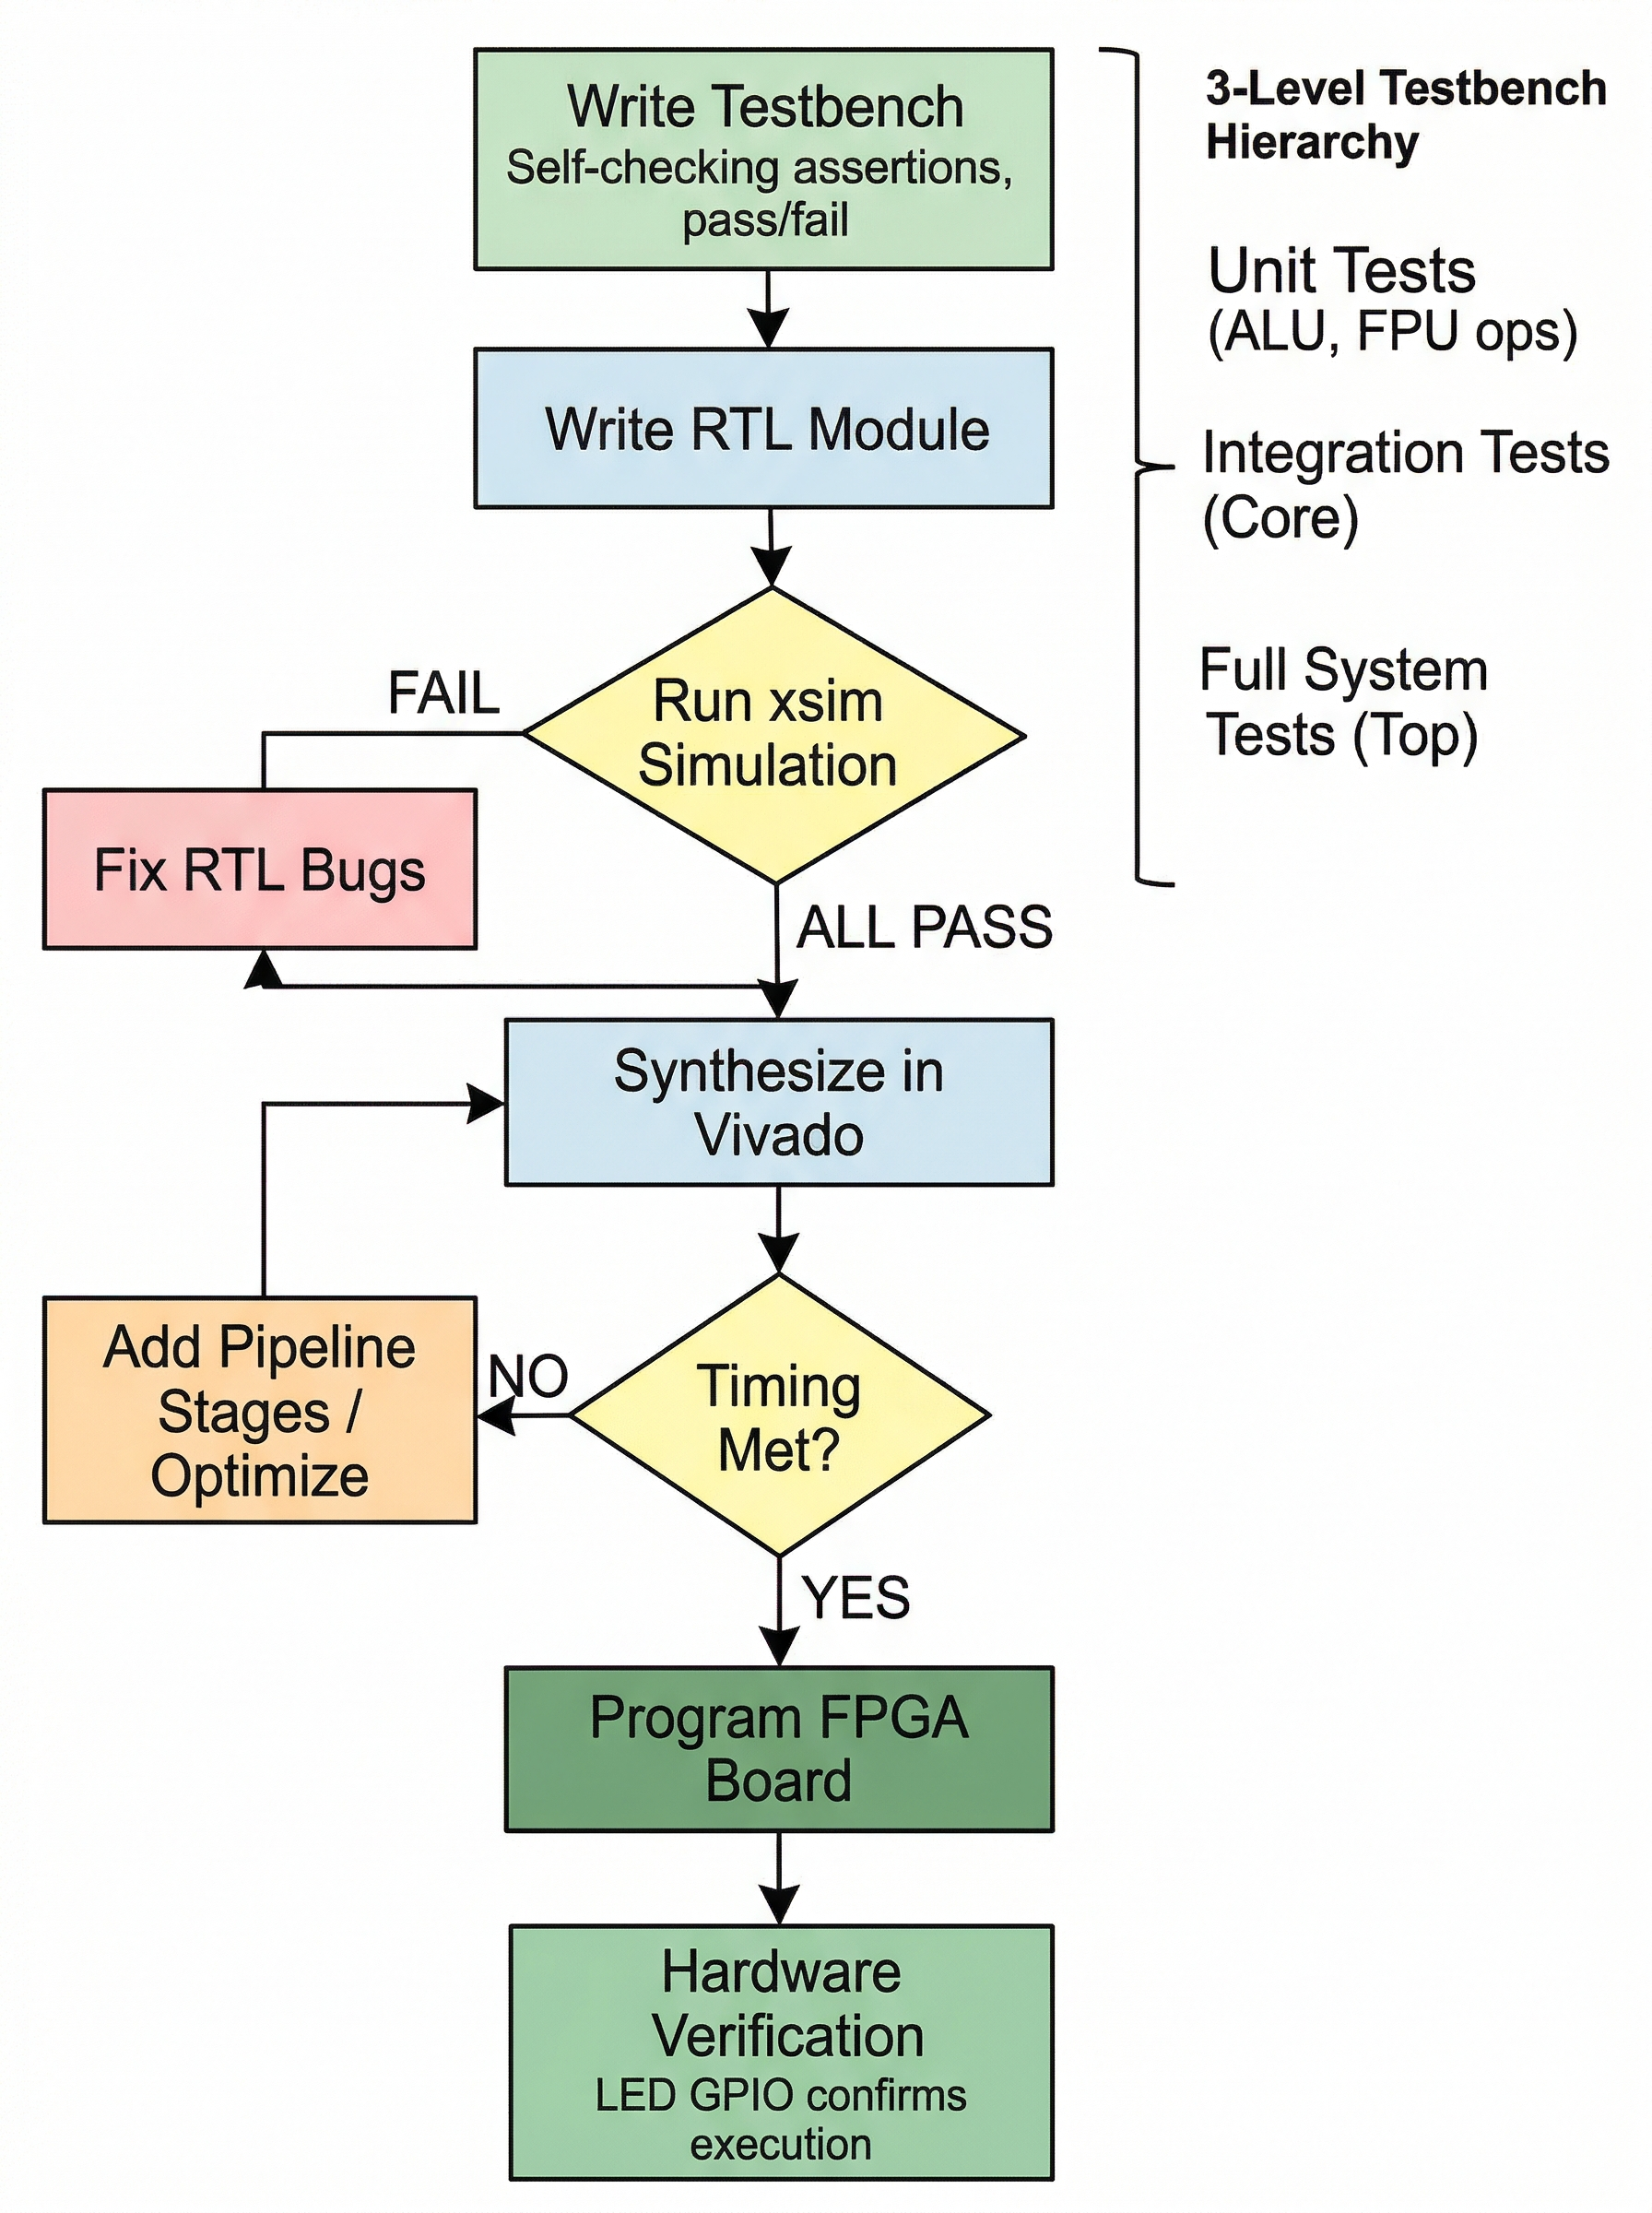
\includegraphics[width=0.7\columnwidth]{figures/fig_tdd_flow.jpg}
\caption{Simulation-first verification workflow enforced by the custom FPGA skill.}
\label{fig:tdd_flow}
\end{figure}

\subsection{Target Platform}

All designs target the Digilent Basys~3 board~\cite{digilent2021basys3}, which is built around a Xilinx Artix-7 XC7A35T FPGA. The device provides 20{,}800 LUTs, 41{,}600 flip-flops, 90~DSP48E1 slices, and 50~36Kb block RAMs~\cite{xilinx2020ds180}. Synthesis, implementation, and bitstream generation used Xilinx Vivado 2020.2~\cite{xilinx2020ug901}. The board operates at a native 100~MHz clock frequency. Hardware verification employed the 16-LED array available on the Basys~3 through memory-mapped GPIO.

\subsection{Formal Verification Methodology}

Formal verification with SystemVerilog Assertions (SVA) complements testing based on simulation. Simulation gives coverage-based confidence through specific test vectors, while formal verification uses satisfiability modulo theories (SMT) solvers to prove that design properties hold for every input combination within a bounded number of clock cycles~\cite{wolf2016symbiyosys}. The two are complementary: simulation catches functional bugs quickly and cheaply, formal verification proves the absence of specific bug classes within the bounded depth.

The formal infrastructure comprises 16 SVA modules totaling roughly 1,500 lines of assertion code, organized into six property categories: (1)~protocol correctness, verifying handshake busy/done sequencing and timing bounds; (2)~ALU functional correctness, checking combinational operation results; (3)~FPU IEEE 754 special-value handling for infinity, NaN, zero, and subnormal operands~\cite{ieee754_2019}; (4)~pipeline forwarding and hazard detection, confirming forwarding priority (EX~$>$~MEM~$>$~WB) and the x0 hardwire invariant~\cite{waterman2019riscv}; (5)~reset synchronizer timing, proving dual-flip-flop metastability invariants; and (6)~memory bus protocol, verifying address-decode mutual exclusion and valid/ready handshaking.

SystemVerilog bind statements attach assertion modules to RTL without touching the generated source~\cite{ieee1800_2017}. This separation keeps the RTL clean and lets either verification approach run on its own. Two engines are supported: SymbiYosys with the Z3 SMT solver for open-source bounded model checking across eight configurations (depths from 1~cycle for combinational ALU checks to 120~cycles for multi-cycle FPU operations), and Vivado xsim for assertion checking during simulation. A Makefile drives both flows, so a single command verifies all properties across the three processor variants.

\section{Implementation}

\subsection{Processor Architecture}

The generated processor family has three tiers. The rv16 design uses a 16-bit datapath with a 3-stage pipeline supporting a 12-instruction subset of the RV32I base integer instruction set architecture (ISA). The rv64 design scales to a 64-bit datapath with a 3-stage pipeline implementing the full 40-instruction RV64I specification. The rv64fp design, the most complex variant, uses a 5-stage pipeline (Fetch, Decode, Execute, Memory, Writeback) and supports the RV64IFD instruction set with 68 instructions.

The rv64fp pipeline uses full data forwarding to resolve read-after-write (RAW) hazards without stalls in the common case. A dedicated hazard-detection unit monitors inter-stage register dependencies and inserts pipeline bubbles for load-use hazards that forwarding cannot resolve. The architecture uses a Harvard memory model with separate instruction and data BRAM, plus memory-mapped GPIO for LED output. Fig.~1 shows the pipeline.

\begin{figure}[!t]
\centering
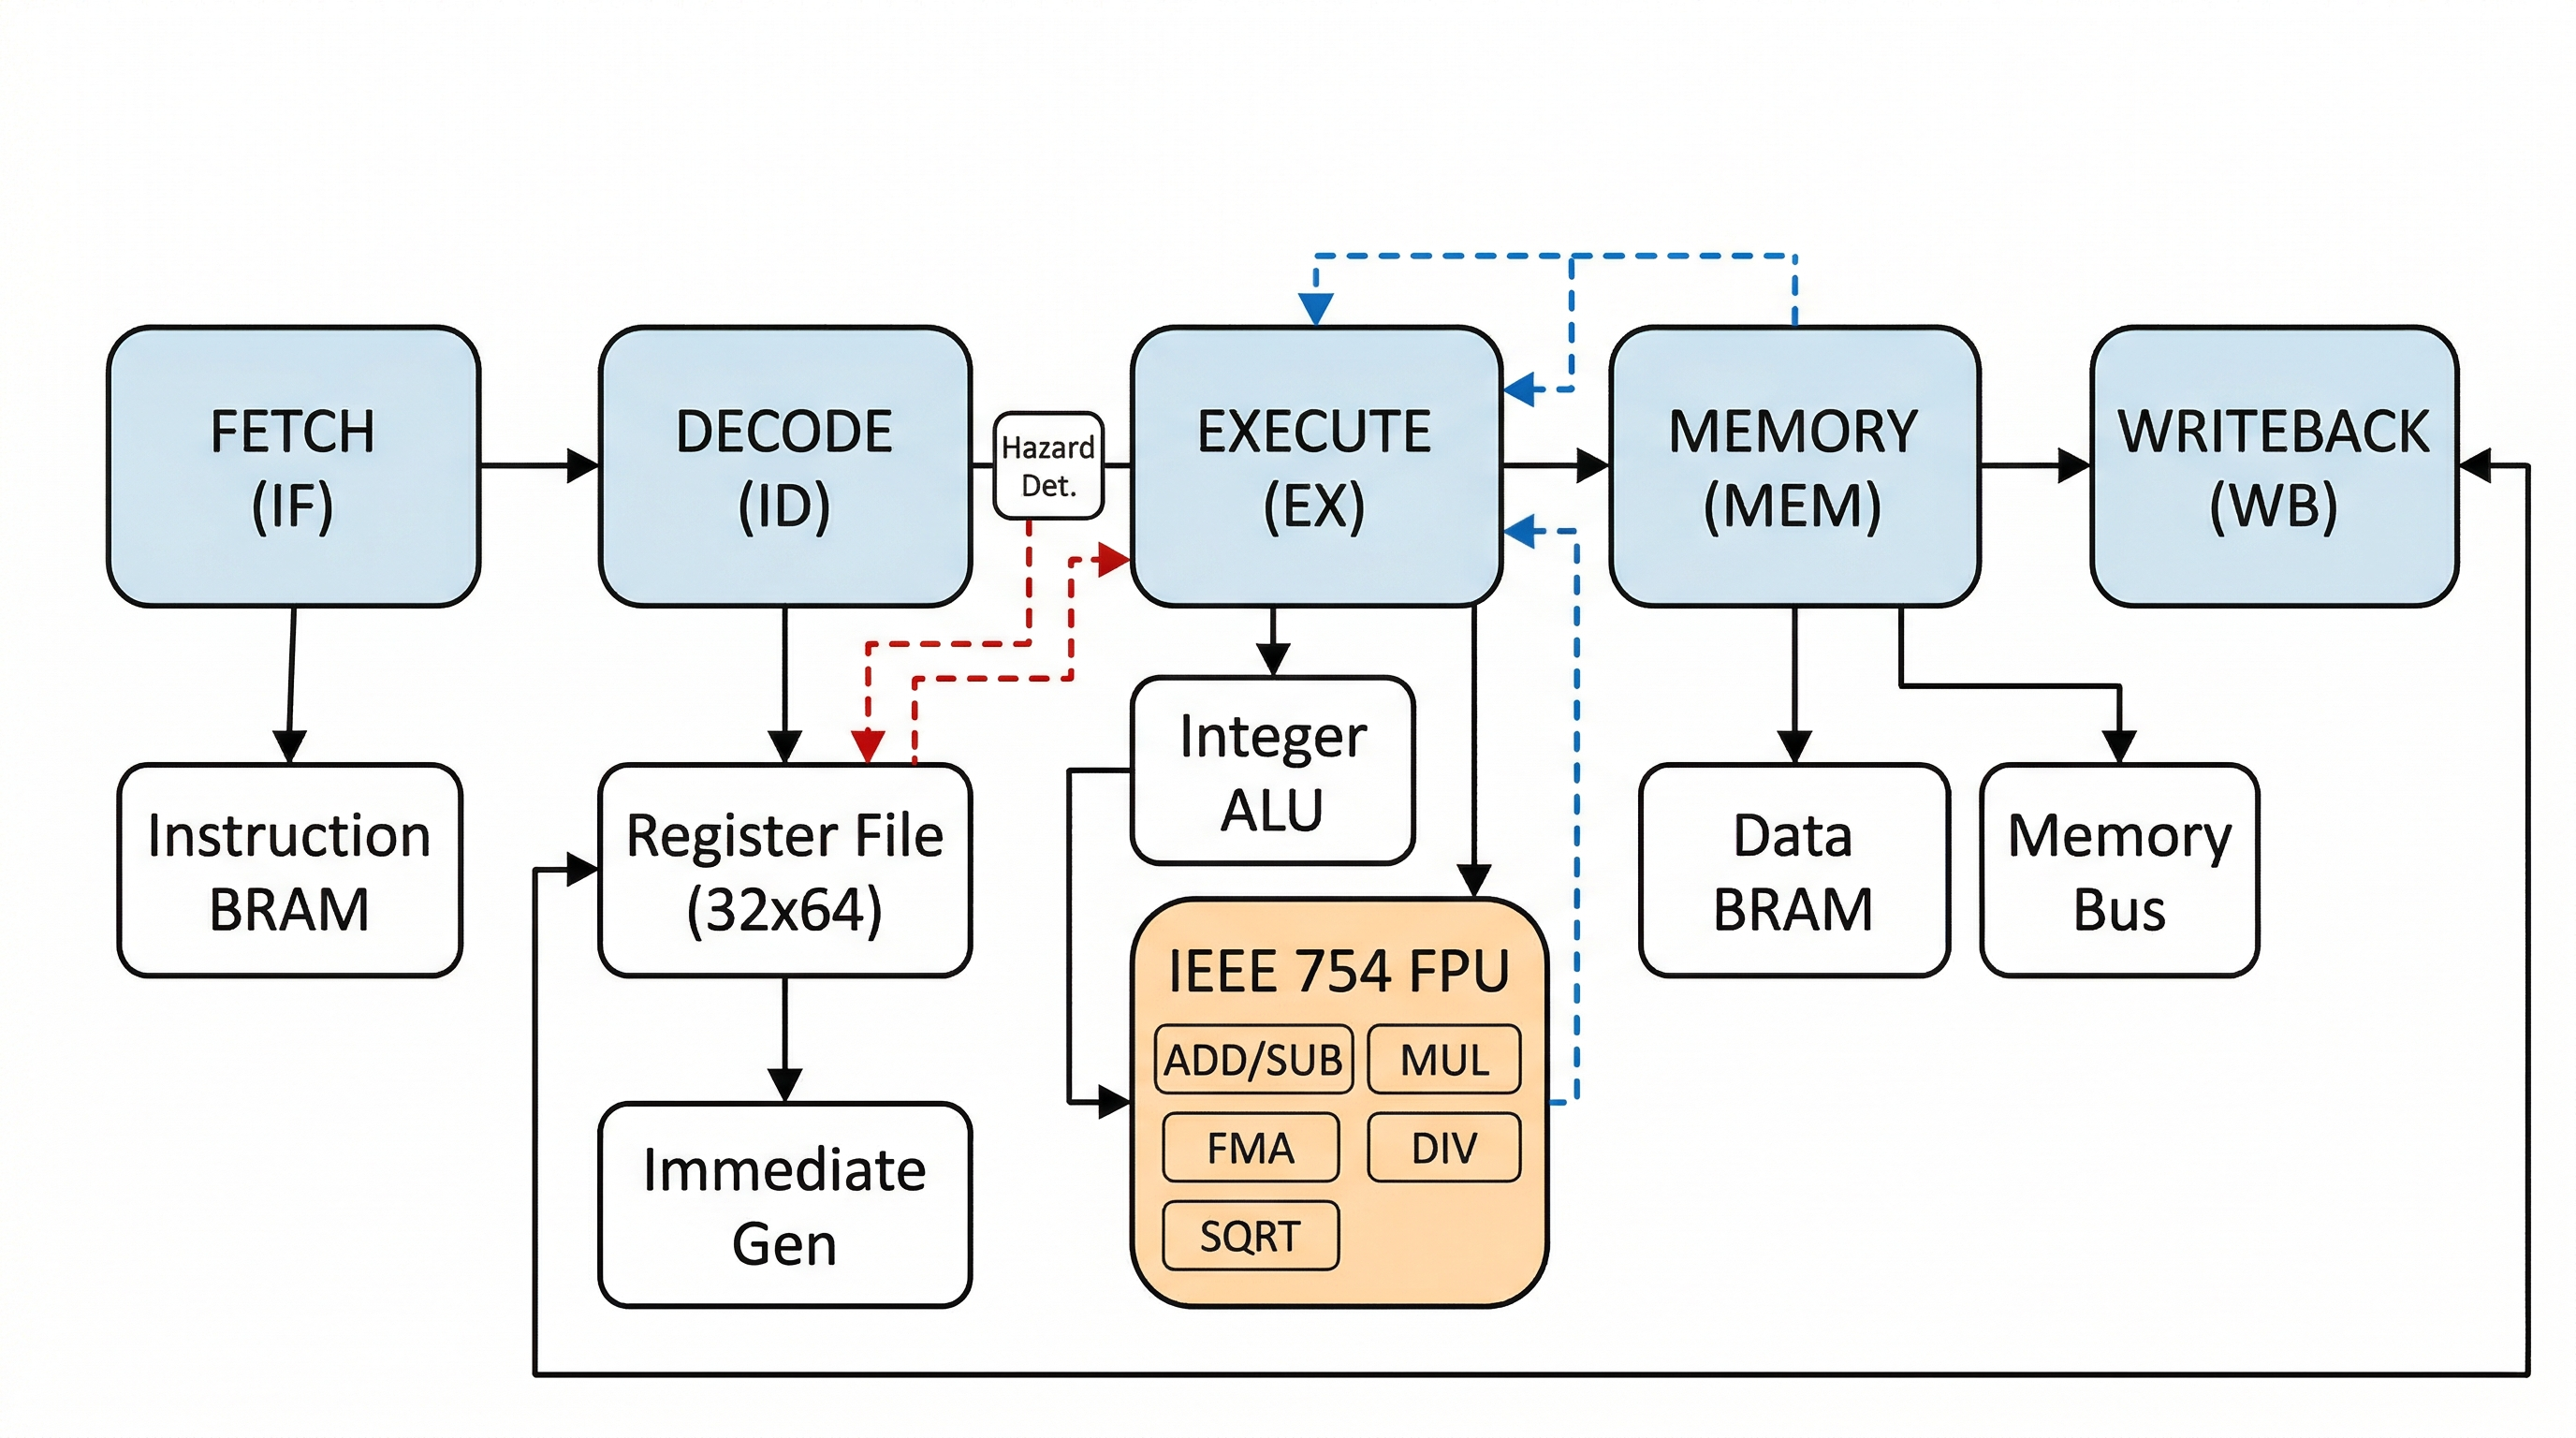
\includegraphics[width=\columnwidth]{figures/fig_pipeline.jpg}
\caption{Five-stage pipeline architecture of the rv64fp processor with IEEE 754 FPU.}
\label{fig:pipeline}
\end{figure}

\subsection{IEEE 754 Floating-Point Unit}

The floating-point unit implements 28 IEEE 754 double-precision operations~\cite{ieee754_2019} across eight specialized execution units. The addition/subtraction unit uses a 3-cycle pipeline with mantissa alignment shifting and leading-zero normalization. The multiplier uses a 3-cycle pipeline with DSP48E1 cascade~\cite{xilinx2020ds180} for full 53-by-53-bit mantissa multiplication. Fused multiply-add (FMA) operations---FMADD, FMSUB, FNMSUB, and FNMADD---skip intermediate rounding and reach higher precision than sequential multiply-then-add. Division and square root are iterative multi-cycle units built on digit-recurrence algorithms.

Other operations cover sign injection (FSGNJ, FSGNJN, FSGNJX), comparisons (FEQ, FLT, FLE) with IEEE 754 NaN handling, classification (FCLASS) for runtime type inspection, and format conversions (FCVT) between integer and floating-point representations in both directions. All five IEEE 754 rounding modes are supported: round to nearest even (RNE), round toward zero (RTZ), round down (RDN), round up (RUP), and round to nearest magnitude (RMM). Each execution unit handles its own special cases: NaN propagation, infinity arithmetic, signed zero, and subnormals.

\subsection{Dual-Language Output}

Each processor variant was generated in both Verilog and VHDL, producing 26 RTL modules per language. The Verilog implementation totals 5,721 lines and the VHDL 4,133. Both variants ship with complete Vivado TCL build scripts for project creation, synthesis, implementation, and bitstream generation, plus shared Basys~3 XDC constraint files for pin mapping and clock definition. Test programs were written in RISC-V assembly and assembled into hexadecimal memory initialization files by a Python script.

\section{Results}

\subsection{Design Metrics}

Table~\ref{tab:design_metrics} summarizes design metrics for the six variants. The designs span three orders of magnitude in complexity, from the 400-LUT rv16 educational core to the 12,969-LUT rv64fp processor with floating-point support.

\begin{table}[!t]
\caption{Design Metrics for All Processor Variants}
\label{tab:design_metrics}
\centering
\resizebox{\columnwidth}{!}{%
\begin{tabular}{lllllrl}
\toprule
Processor & Language & Datapath & Pipeline & ISA & Instr. & LUTs \\
\midrule
rv16   & Verilog & 16-bit & 3-stage & RV32I sub. & 12 & $\sim$400 \\
rv64   & Verilog & 64-bit & 3-stage & RV64I      & 40 & 3,273 \\
rv64fp & Verilog & 64-bit & 5-stage & RV64IFD    & 68 & 12,969 \\
rv16   & VHDL    & 16-bit & 3-stage & RV32I sub. & 12 & $\sim$400 \\
rv64   & VHDL    & 64-bit & 3-stage & RV64I      & 40 & 3,273 \\
rv64fp & VHDL    & 64-bit & 5-stage & RV64IFD    & 68 & 12,969 \\
\bottomrule
\end{tabular}%
}
\end{table}

\subsection{Verification Results}

The simulation-first framework caught 10 bugs in the initial FPU generation: rounding edge cases in the addition/subtraction unit where guard, round, and sticky bit computation failed for certain mantissa alignments; NaN propagation errors in the comparison unit that did not distinguish quiet from signaling NaN per IEEE 754 Section 6.2~\cite{ieee754_2019}; and a sign-bit inversion in FNMSUB that negated the wrong intermediate.

Unit-level testbenches (tb\_alu.v and tb\_fpu\_ops.v) verified each ALU and FPU operation in isolation. The tb\_fpu\_ops.v testbench runs 327 lines and exercises all 28 FPU operations with IEEE 754 test constants: positive and negative zero, infinity, quiet NaN, signaling NaN, and subnormal values. Each test case carries a descriptive label for immediate failure identification in logs, plus timeout protection to catch infinite loops in the iterative division and square root units.

Integration-level testbenches (tb\_rv16\_core.v) loaded test programs via \$readmemh, instantiated dual-port memory models, and checked program counter progression and register file state across multi-instruction sequences. These reached hazard-detection and data-forwarding bugs that unit-level testing could not. System-level testbenches (tb\_rv64fp\_full.v) ran complete test programs for more than 2{,}000 simulation cycles and mapped FPU results to LED bit positions for hardware correlation.

SymbiYosys bounded model checking proved correctness properties across all three variants. Table~\ref{tab:formal_results} lists the results by property category. For rv64fp, BMC at depth 120 proved FPU protocol correctness: the busy/done handshake invariant, eventual completion within bounded cycles, and IEEE 754 special-value handling for all five arithmetic operations. ALU properties were proved at depth 1 through combinational checking. Pipeline hazard-detection properties confirmed forwarding priority and the x0 hardwire invariant at depth 10. Memory bus properties verified address-decode mutual exclusion and valid/ready protocol compliance.

The formal runs confirmed the absence of protocol violations reachable within the bounded depths. The FPU IEEE 754 properties covered NaN propagation, infinity arithmetic, and exception flag generation on edge cases that simulation would need impractically large suites to exhaust. The bind approach added formal verification without touching any of the 26 RTL modules per language, preserving the simulation-verified designs.

\begin{table}[!t]
\caption{Formal Verification Results by Property Category}
\label{tab:formal_results}
\centering
\resizebox{\columnwidth}{!}{%
\begin{tabular}{llllc}
\toprule
Property Category & Variants & Engine & Depth & Status \\
\midrule
ALU Correctness      & rv16, rv64, rv64fp & SymbiYosys BMC & 1   & PASS \\
FPU Protocol         & rv64fp             & SymbiYosys BMC & 120 & PASS \\
FPU IEEE 754         & rv64fp             & SymbiYosys BMC & 120 & PASS \\
Hazard Detection     & rv64fp             & SymbiYosys BMC & 10  & PASS \\
Reset Synchronizer   & rv16, rv64, rv64fp & SymbiYosys BMC & 10  & PASS \\
Memory Bus Protocol  & rv64fp             & SymbiYosys BMC & 10  & PASS \\
\bottomrule
\end{tabular}%
}
\end{table}

\begin{figure}[!t]
\centering
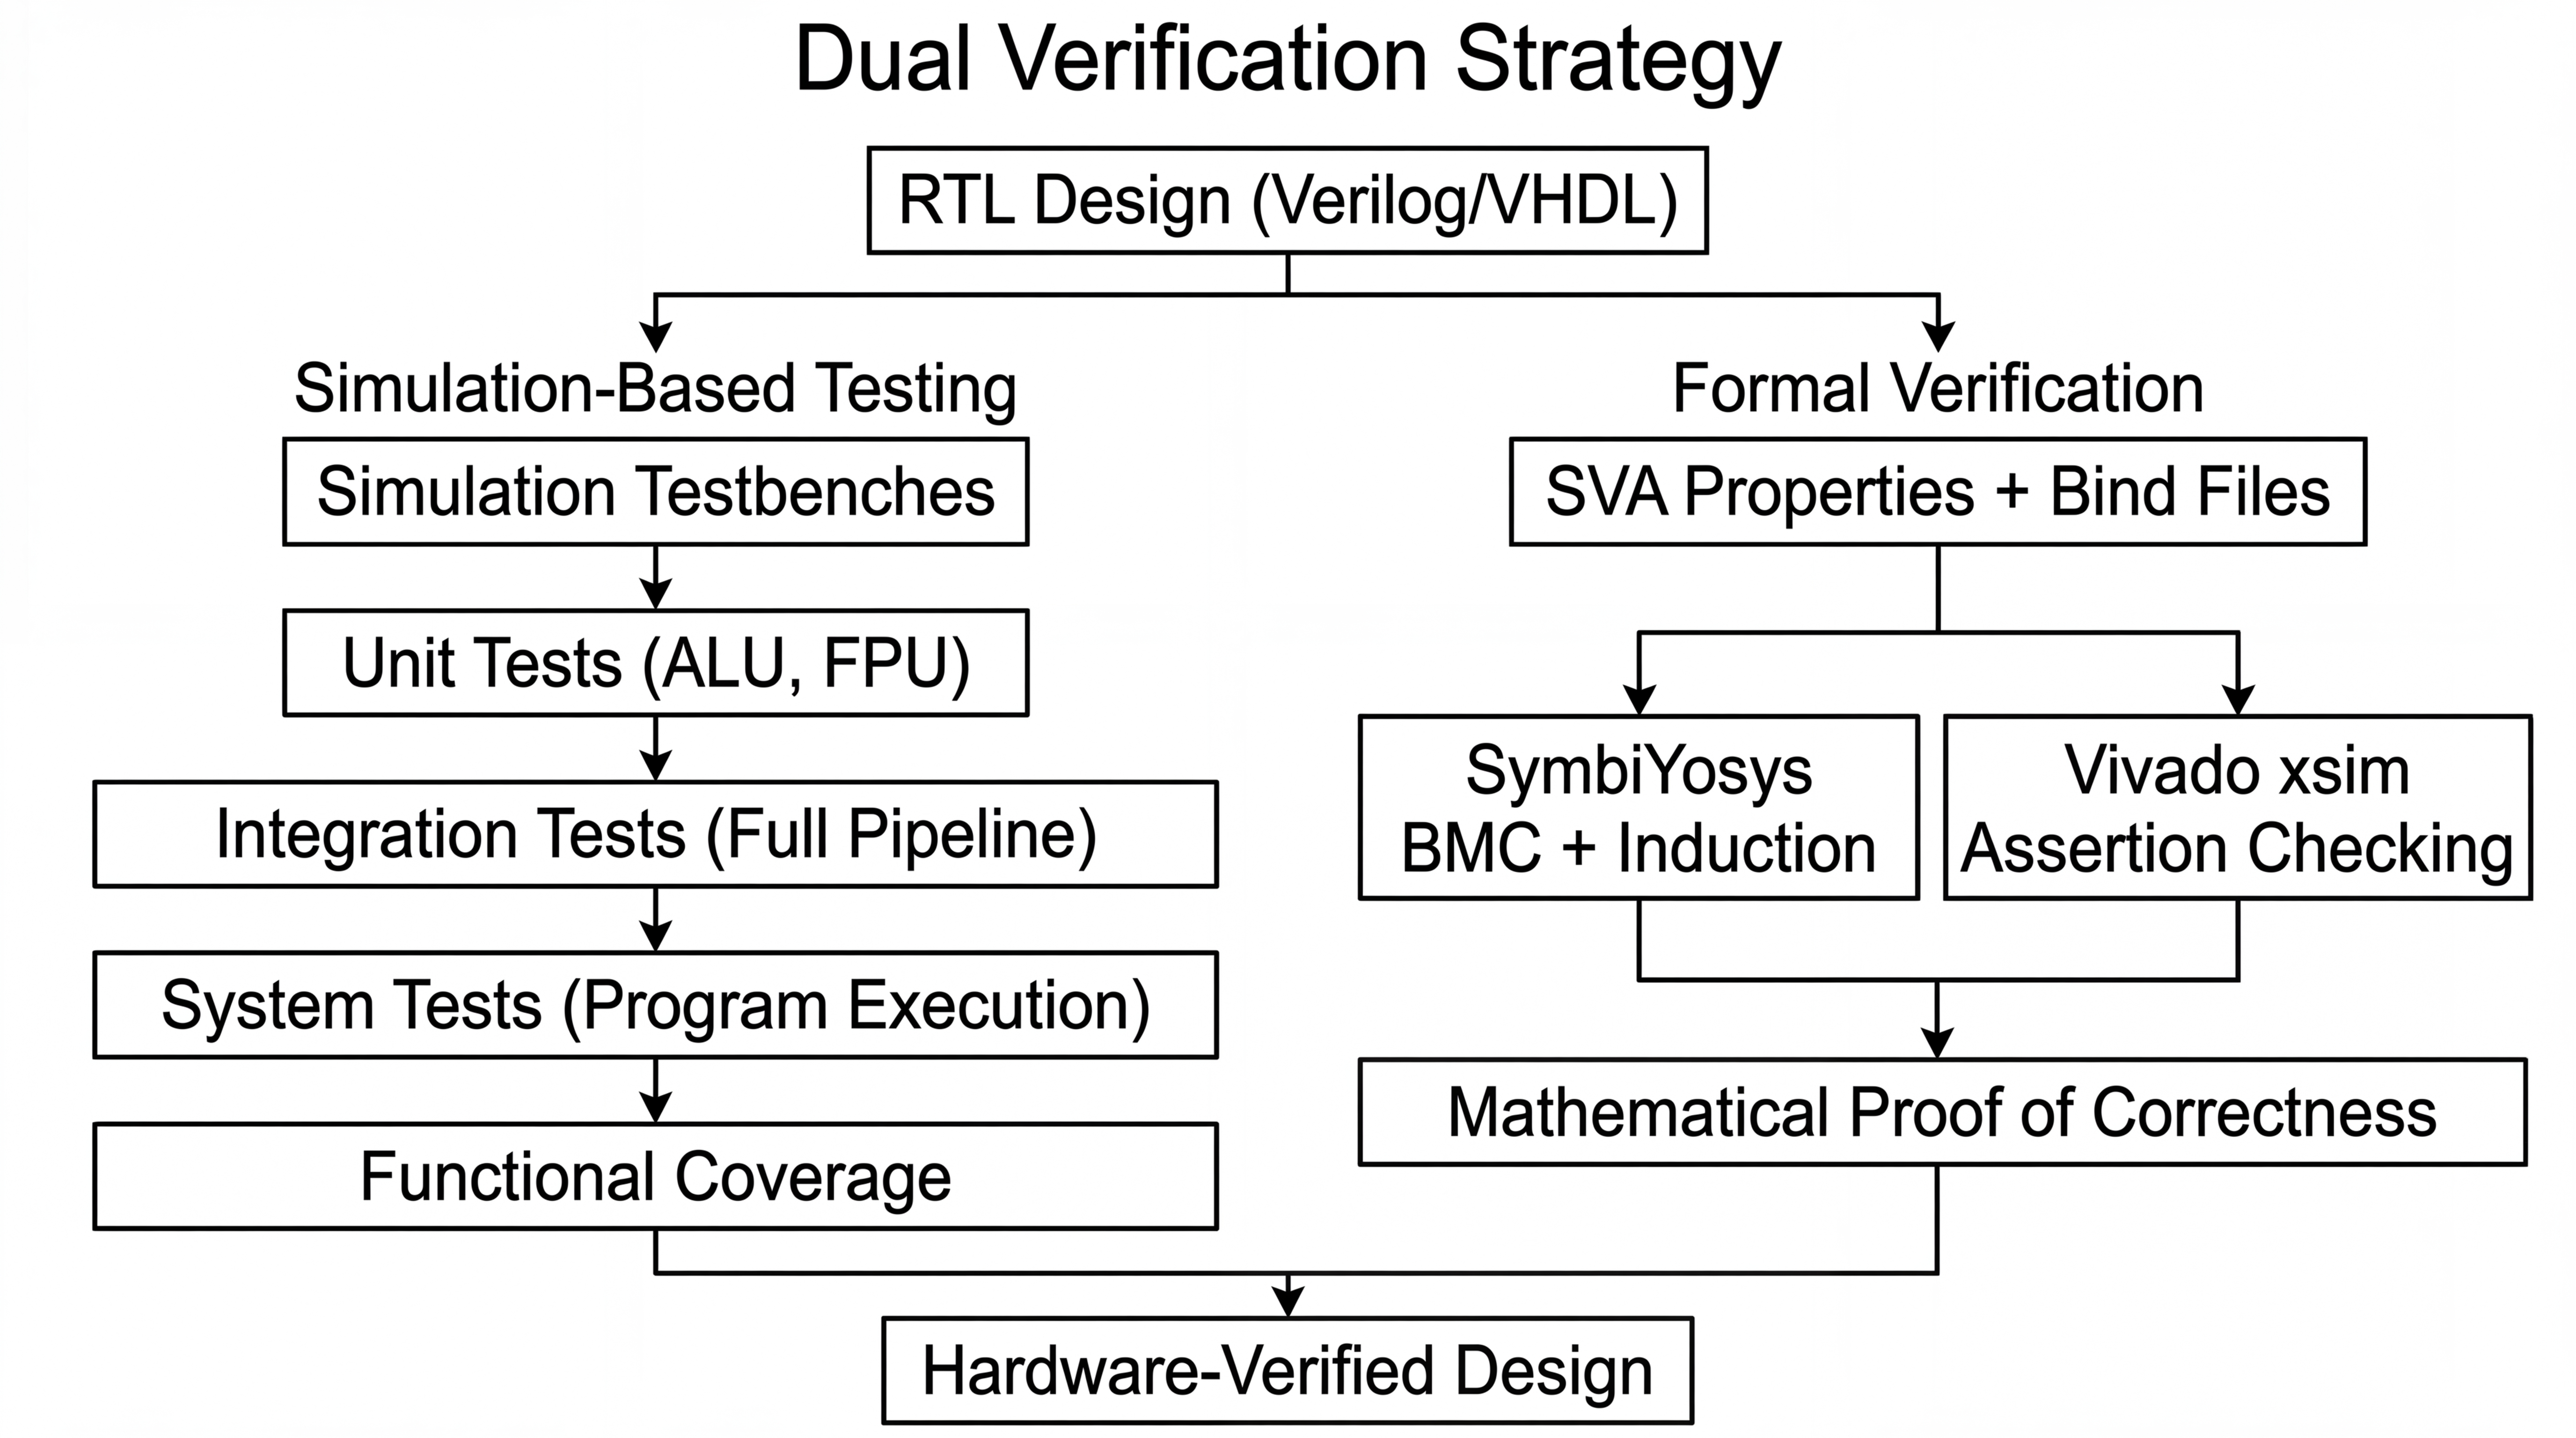
\includegraphics[width=\columnwidth]{figures/fig_verification_strategy.jpg}
\caption{Complementary verification strategy combining simulation-based testing and SVA formal verification.}
\label{fig:verification_strategy}
\end{figure}

\subsection{Resource Optimization}

The simulation-driven flow cut resource use significantly. The fp\_fma module, which implements fused multiply-add, dropped from 13{,}932 LUTs to 1{,}942 LUTs, an 86\% reduction. The full rv64fp system fell from roughly 25{,}000 LUTs to 12{,}969 LUTs, a 48\% reduction overall. Fig.~4 shows the LUT utilization before and after.

Explicit resource-minimization techniques were not used. The reduction came from the simulation-first workflow itself. Testbenches pinned down the exact functional requirements for each module, and dead logic paths and redundant special-case handling then became visible and were removed. The FMA unit, for example, carried elaborate exception handling for cases that upstream modules had already handled. Once simulation showed those cases could not reach it, the redundant logic was deleted.

The final rv64fp design consumes 12,969 of the 20,800 LUTs on the XC7A35T (82.9\% utilization) and 18 of the 90 DSP48E1 slices for mantissa multiplication in the floating-point multiplier and FMA units.

\begin{figure}[!t]
\centering
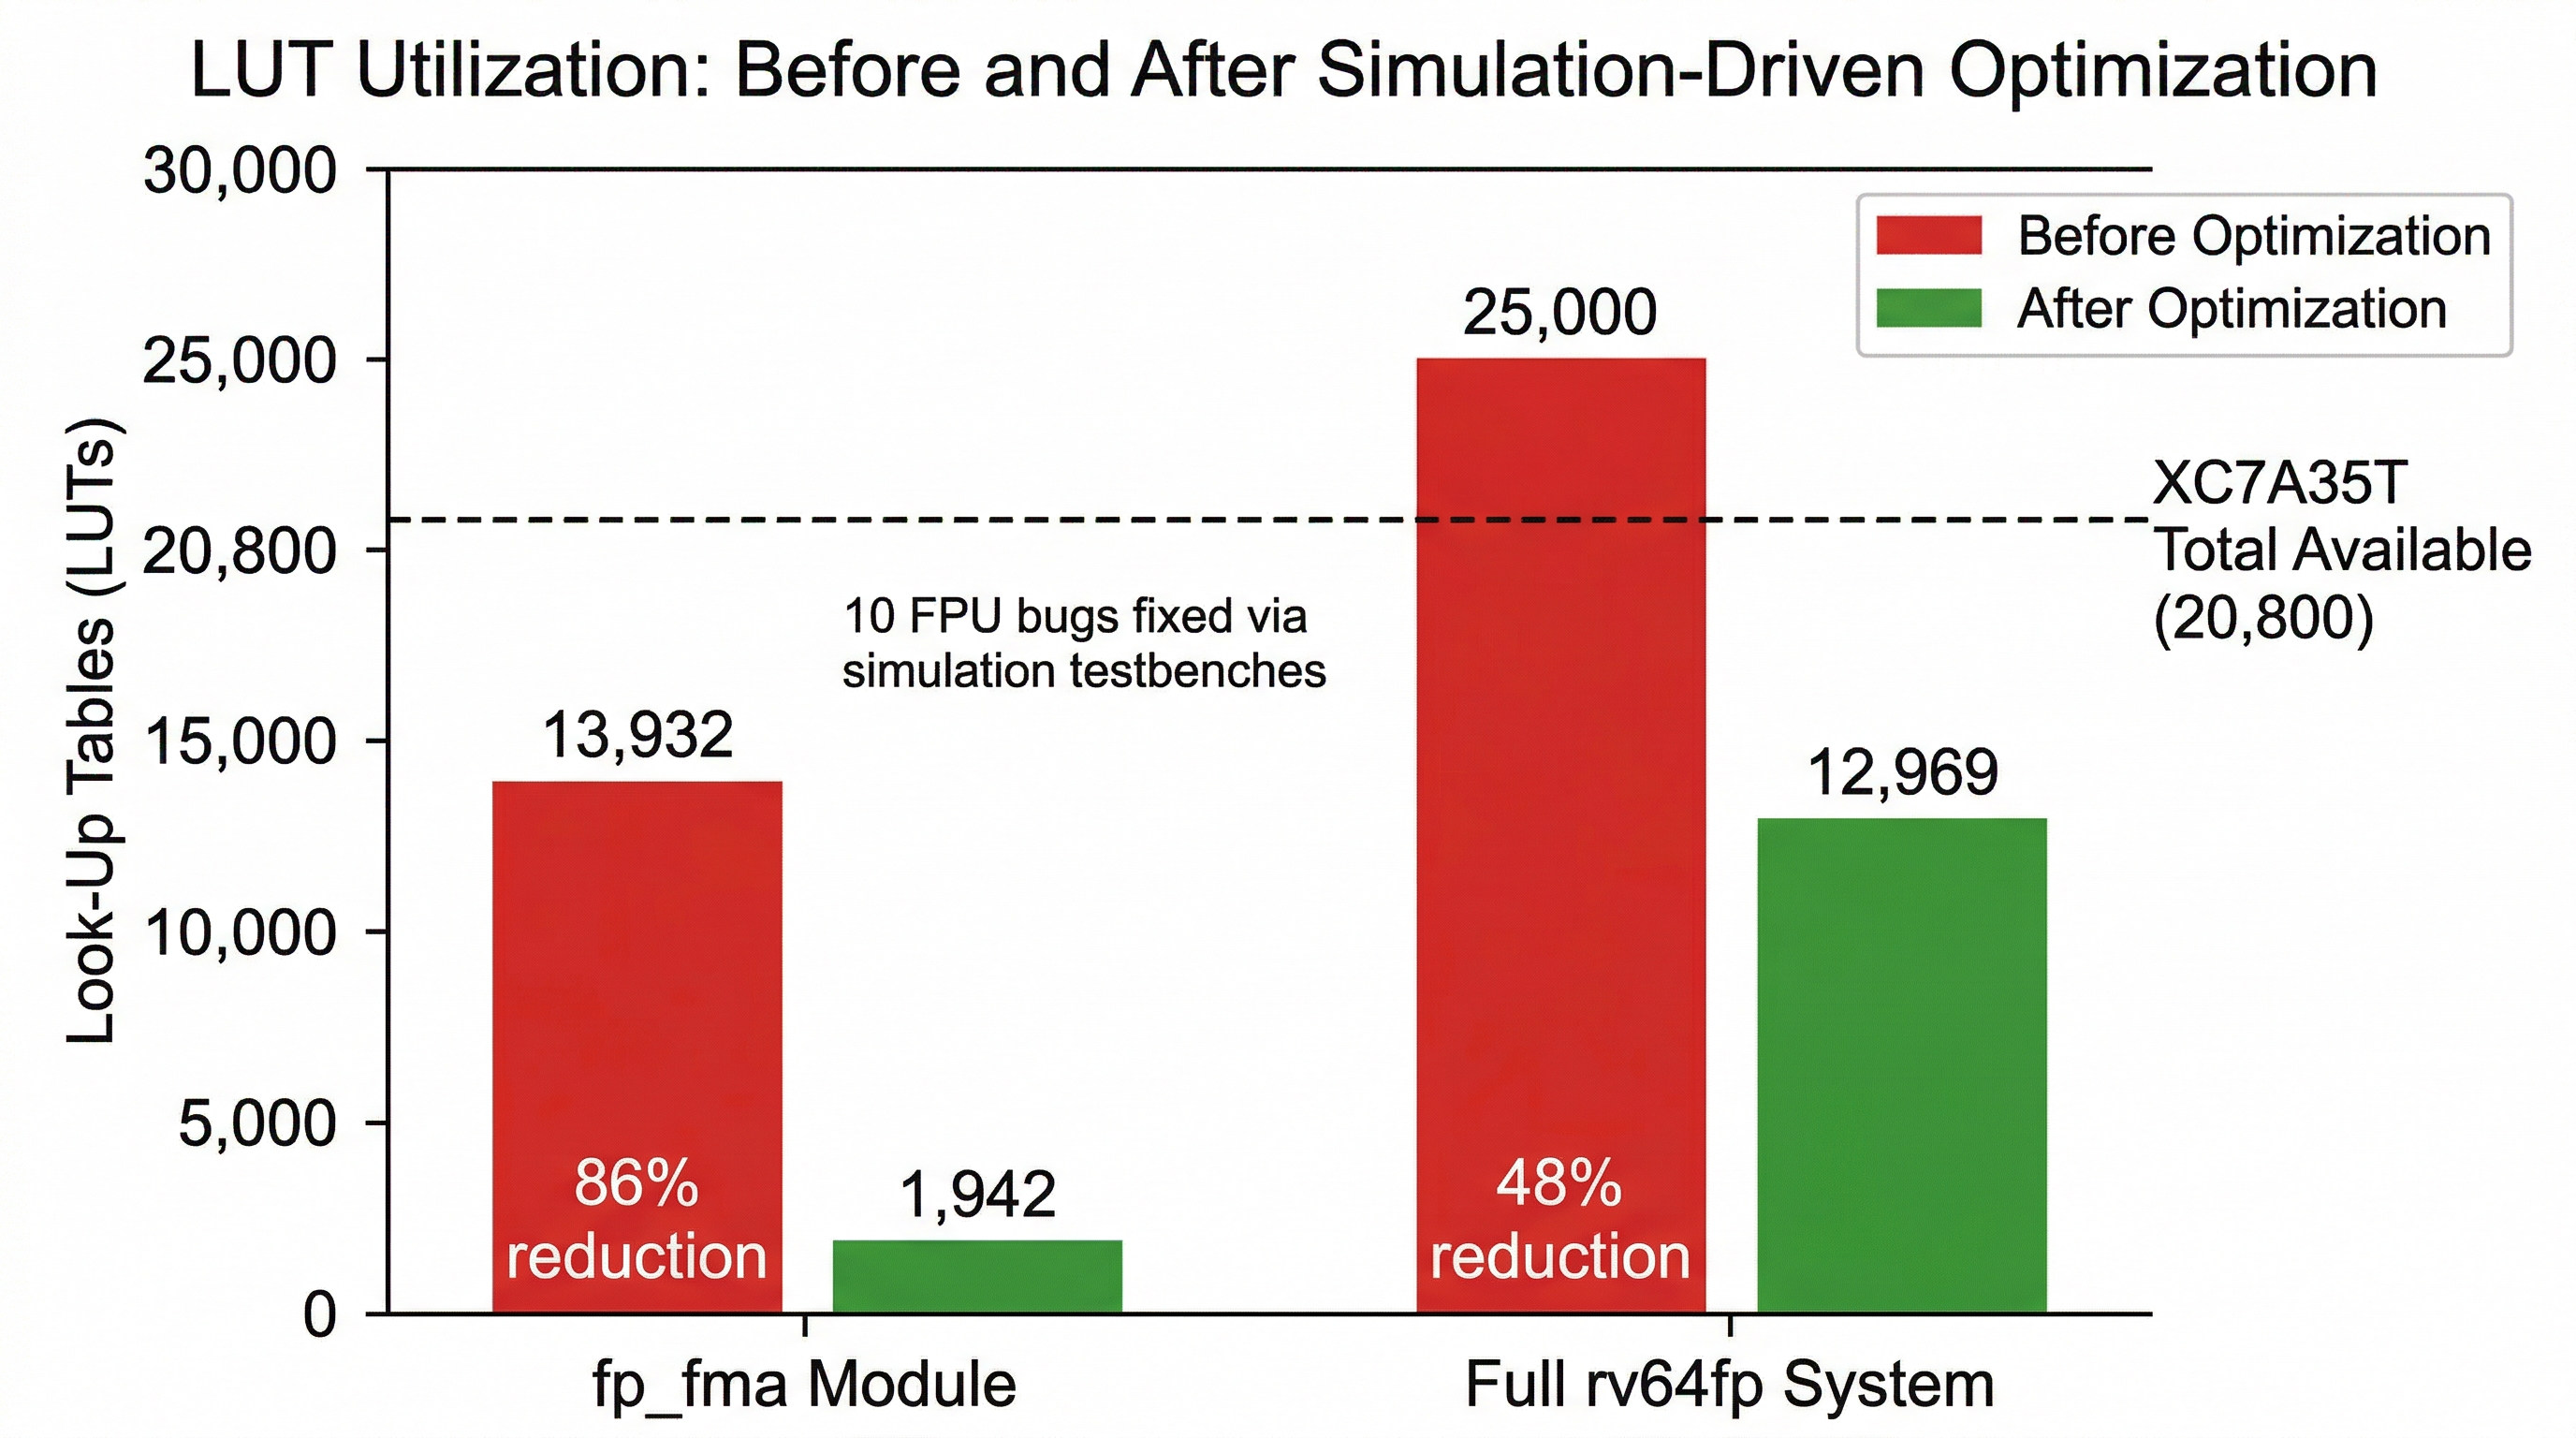
\includegraphics[width=\columnwidth]{figures/fig_lut_optimization.jpg}
\caption{LUT utilization before and after simulation-driven optimization.}
\label{fig:lut_optimization}
\end{figure}

\subsection{Hardware Verification on Basys 3}

All six variants were verified on a Digilent Basys 3 development board~\cite{digilent2021basys3} running at the board's native 100~MHz clock under Vivado 2020.2~\cite{xilinx2020ug901}. Hardware verification used the memory-mapped GPIO interface. Test programs ran on each processor and wrote results to the LED output register; each of the 16 LED bits carried the pass/fail status of a specific test covering ALU operations, branches, load/store behavior, and individual FPU operations.

The simple hardware strategy worked because the simulation coverage was exhaustive. Simulation testbenches already covered functional correctness, so the hardware test only needed to confirm that the synthesized netlist matched the simulation model. No discrepancies between simulation and hardware appeared for any of the six designs.

\section{Discussion}

Skill-based context engineering raises the quality of AI-generated HDL materially. Without the skill, the base model produces generic Verilog with no simulation infrastructure, no version awareness, and no systematic treatment of IEEE 754 special cases. The skill supplies domain expertise the model lacks: clock-domain crossing patterns, pipeline design with forwarding, BRAM inference rules, and DSP48E1 utilization strategies for the Xilinx 7-series architecture~\cite{xilinx2020ds180}.

The simulation-first TDD mandate was the most consequential piece of the skill architecture. The 10 bugs caught in the initial FPU generation would have been much harder to diagnose after synthesis. More important, simulation drove a 48\% reduction in LUT utilization by exposing unreachable and redundant logic. This suggests that AI-generated HDL tends to over-provision exception handling when concrete test cases are absent.

The Context7 MCP integration addressed a characteristic failure mode of LLM code generation: confident but incorrect specification of precise technical details. RISC-V instruction encodings require exact bit-field values; a single bad bit in funct7 produces a different instruction entirely~\cite{waterman2019riscv}. IEEE 754 special-case rules are subtle: quiet vs. signaling NaN, the sign of zero in subtraction, the behavior of infinity in division, all have precise specifications the model's training data may not capture~\cite{ieee754_2019}. Live documentation retrieval eliminated this class of error.

\subsection{Comparison with Prior Work}

Table~\ref{tab:comparison} compares this work against prior AI-assisted HDL efforts. The gap is qualitative across datapath width, pipeline depth, instruction count, and verification rigor.

\begin{table}[!t]
\caption{Comparison with Prior Work in AI-Assisted HDL Generation}
\label{tab:comparison}
\centering
\resizebox{\columnwidth}{!}{%
\begin{tabular}{lccccc}
\toprule
\textbf{Metric} & \textbf{DAVE} & \textbf{Chip-Chat} & \textbf{HDLGen} & \textbf{ResBench} & \textbf{This Work} \\
 & \cite{pearce2020dave} & \cite{blocklove2023chipchat} & \cite{sun2024hdlgen} & \cite{zhao2025resbench} & \\
\midrule
Year           & 2020    & 2023     & 2024    & 2025    & 2026 \\
LLM            & GPT-2   & GPT-4    & GPT-3.5 & Various & Claude Opus 4.6 \\
Datapath       & N/A     & 8-bit    & 32-bit  & Module  & 64-bit \\
Pipeline       & None    & None     & N/A     & N/A     & 5-stage \\
FPU            & No      & No       & No      & No      & IEEE 754 DP \\
Instructions   & N/A     & $\sim$10 & 40      & N/A     & 68 \\
Dual Language  & No      & No       & Yes     & No      & Yes \\
Verification   & N/A     & Manual   & Sim     & Sim     & TDD + SVA \\
Formal Verif.  & No      & No       & No      & No      & SymbiYosys \\
HDL Lines      & $\sim$100 & $\sim$500 & $\sim$2,000 & Varies & 9,854 \\
\bottomrule
\end{tabular}%
}
\end{table}

The main differentiator is the IEEE 754 double-precision FPU. No prior AI-generated HDL has attempted floating-point arithmetic, which requires careful handling of subnormals, NaN propagation, infinity arithmetic, signed-zero semantics, and five rounding modes. The 28 FPU operations here represent a class of hardware that demands exact compliance with a formal specification---a stringent test of AI-assisted design.

Verification is the other categorical shift. Prior work relied on manual inspection~\cite{blocklove2023chipchat} or simulation alone~\cite{sun2024hdlgen, zhao2025resbench}. This work combines simulation-based TDD with SVA and SymbiYosys bounded model checking, giving mathematical guarantees about protocol correctness and IEEE 754 compliance within bounded depths. The bind-based infrastructure stays separate from the generated RTL, so verification runs without modifying the AI-generated source.

The 50$\times$ jump in HDL line count---from $\sim$500 lines for Chip-Chat's 8-bit processor to 9,854 lines across both languages---is not just size. It reflects a 5-stage pipeline with data forwarding, hazard detection, and a multi-unit FPU with iterative division and square root. Skill-based context engineering enables the leap by front-loading the knowledge prior approaches expected the model to possess inherently.

Several limitations apply. The formal proofs are bounded to finite depths (up to 120 cycles for FPU operations) and do not constitute unbounded correctness proofs. The designs run at the Basys~3 board's native 100~MHz; timing closure at higher frequencies has not been attempted. The 48\% resource reduction is large, but no comparison against manually optimized designs by experienced engineers was performed.

The combination of simulation and formal verification shows the value of a multi-modal strategy for AI-generated HDL. Simulation handles rapid functional debugging and regression; formal methods guarantee protocol adherence and invariant preservation. The bind methodology keeps the formal infrastructure separate from the generated RTL, so either approach runs independently without modifying the designs---valuable for AI-generated code, where regeneration can overwrite manual changes.

\section{Conclusion}

This paper presented a skill-based methodology for AI-assisted RISC-V processor design. Six complete, hardware-verified variants came out of a single generation session. The custom FPGA skill merges community-contributed design knowledge with simulation-first TDD, formal verification through SVA, live documentation retrieval, and Vivado version awareness. It enabled one-shot generation of designs from a 12-instruction educational core to a 68-instruction RV64IFD processor with an IEEE 754 double-precision FPU.

The simulation-first framework caught 10 FPU bugs in the initial generation and drove a 48\% LUT reduction, from roughly 25,000 to 12,969 LUTs. Formal verification then proved correctness properties across six categories via SymbiYosys bounded model checking, confirming protocol compliance, ALU and FPU functional correctness, and pipeline hazard detection. The most complex design uses 82.9\% of the available LUTs on the Xilinx Artix-7 XC7A35T and was verified on a Digilent Basys 3 board at 100~MHz. Dual-language output covers 26 RTL modules per language, totaling 5,721 lines of Verilog and 4,133 lines of VHDL.

Two directions remain for future work. First, unbounded induction proofs for critical properties, possibly through abstract models or assume-guarantee decomposition to manage the 64-bit state space. Second, extension to more complex designs---multi-core processors, cache hierarchies, and high-speed serial interfaces---to map the boundaries of skill-based AI-assisted hardware design.

\section*{AI Tool Disclosure}
This work used Claude Code (Anthropic, 2026) as an AI coding assistant for HDL generation. All generated code was verified through simulation testbenches, formal verification, and hardware testing as described in Sections~II and~IV. The manuscript was prepared by the authors.

\section*{Acknowledgment}
The authors thank the University of New Mexico Department of Electrical and Computer Engineering for institutional support. No external funding supported this work.

\clearpage
\bibliographystyle{IEEEtran}
\bibliography{references_tcad}

\end{document}
